

\tikzset{every picture/.style={line width=0.75pt}} %set default line width to 0.75pt        

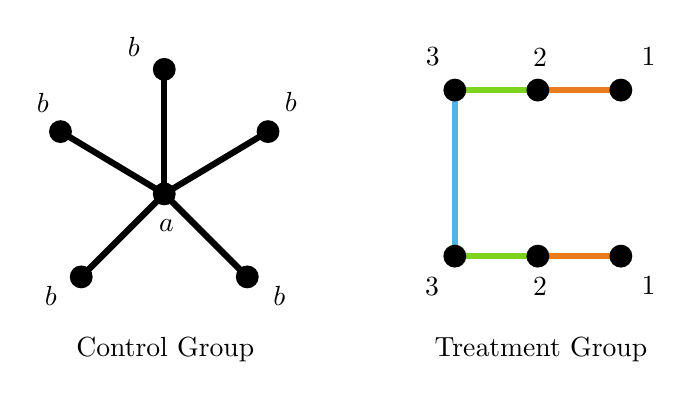
\begin{tikzpicture}[x=0.75pt,y=0.75pt,yscale=-1,xscale=1]
	%uncomment if require: \path (0,242); %set diagram left start at 0, and has height of 242
	
	%Straight Lines [id:da8360249781061426] 
	\draw [color={rgb, 255:red, 235; green, 124; blue, 29 }  ,draw opacity=1 ][line width=2.25]    (285,155) -- (325,155) ;
	%Straight Lines [id:da8158257704190623] 
	\draw [color={rgb, 255:red, 235; green, 124; blue, 29 }  ,draw opacity=1 ][line width=2.25]    (285,75) -- (325,75) ;
	%Straight Lines [id:da7285129998191696] 
	\draw [line width=2.25]    (105,65) -- (105,125) ;
	%Straight Lines [id:da1945257120538626] 
	\draw [line width=2.25]    (65,165) -- (105,125) ;
	%Straight Lines [id:da15064502001286517] 
	\draw [line width=2.25]    (105,125) -- (145,165) ;
	%Straight Lines [id:da8625361583469673] 
	\draw [color={rgb, 255:red, 126; green, 211; blue, 33 }  ,draw opacity=1 ][line width=2.25]    (245,75) -- (285,75) ;
	%Straight Lines [id:da8513199064736671] 
	\draw [color={rgb, 255:red, 126; green, 211; blue, 33 }  ,draw opacity=1 ][line width=2.25]    (245,155) -- (285,155) ;
	%Straight Lines [id:da5064308868951334] 
	\draw [color={rgb, 255:red, 80; green, 181; blue, 227 }  ,draw opacity=1 ][line width=2.25]    (245,75) -- (245,155) ;
	%Shape: Circle [id:dp7020190518871161] 
	\draw  [fill={rgb, 255:red, 0; green, 0; blue, 0 }  ,fill opacity=1 ] (100,65) .. controls (100,62.24) and (102.24,60) .. (105,60) .. controls (107.76,60) and (110,62.24) .. (110,65) .. controls (110,67.76) and (107.76,70) .. (105,70) .. controls (102.24,70) and (100,67.76) .. (100,65) -- cycle ;
	%Shape: Circle [id:dp4472245437398714] 
	\draw  [fill={rgb, 255:red, 0; green, 0; blue, 0 }  ,fill opacity=1 ] (100,125) .. controls (100,122.24) and (102.24,120) .. (105,120) .. controls (107.76,120) and (110,122.24) .. (110,125) .. controls (110,127.76) and (107.76,130) .. (105,130) .. controls (102.24,130) and (100,127.76) .. (100,125) -- cycle ;
	%Shape: Circle [id:dp332527728107481] 
	\draw  [fill={rgb, 255:red, 0; green, 0; blue, 0 }  ,fill opacity=1 ] (60,165) .. controls (60,162.24) and (62.24,160) .. (65,160) .. controls (67.76,160) and (70,162.24) .. (70,165) .. controls (70,167.76) and (67.76,170) .. (65,170) .. controls (62.24,170) and (60,167.76) .. (60,165) -- cycle ;
	%Shape: Circle [id:dp5070907001685069] 
	\draw  [fill={rgb, 255:red, 0; green, 0; blue, 0 }  ,fill opacity=1 ] (140,165) .. controls (140,162.24) and (142.24,160) .. (145,160) .. controls (147.76,160) and (150,162.24) .. (150,165) .. controls (150,167.76) and (147.76,170) .. (145,170) .. controls (142.24,170) and (140,167.76) .. (140,165) -- cycle ;
	%Shape: Circle [id:dp7312361016882203] 
	\draw  [fill={rgb, 255:red, 0; green, 0; blue, 0 }  ,fill opacity=1 ] (240,75) .. controls (240,72.24) and (242.24,70) .. (245,70) .. controls (247.76,70) and (250,72.24) .. (250,75) .. controls (250,77.76) and (247.76,80) .. (245,80) .. controls (242.24,80) and (240,77.76) .. (240,75) -- cycle ;
	%Shape: Circle [id:dp6877519316777763] 
	\draw  [fill={rgb, 255:red, 0; green, 0; blue, 0 }  ,fill opacity=1 ] (320,75) .. controls (320,72.24) and (322.24,70) .. (325,70) .. controls (327.76,70) and (330,72.24) .. (330,75) .. controls (330,77.76) and (327.76,80) .. (325,80) .. controls (322.24,80) and (320,77.76) .. (320,75) -- cycle ;
	%Shape: Circle [id:dp21492882036619276] 
	\draw  [fill={rgb, 255:red, 0; green, 0; blue, 0 }  ,fill opacity=1 ] (320,155) .. controls (320,152.24) and (322.24,150) .. (325,150) .. controls (327.76,150) and (330,152.24) .. (330,155) .. controls (330,157.76) and (327.76,160) .. (325,160) .. controls (322.24,160) and (320,157.76) .. (320,155) -- cycle ;
	%Shape: Circle [id:dp1595771278608995] 
	\draw  [fill={rgb, 255:red, 0; green, 0; blue, 0 }  ,fill opacity=1 ] (240,155) .. controls (240,152.24) and (242.24,150) .. (245,150) .. controls (247.76,150) and (250,152.24) .. (250,155) .. controls (250,157.76) and (247.76,160) .. (245,160) .. controls (242.24,160) and (240,157.76) .. (240,155) -- cycle ;
	%Straight Lines [id:da9822349173412578] 
	\draw [line width=2.25]    (105,125) -- (155,95) ;
	%Shape: Circle [id:dp7709379434514961] 
	\draw  [fill={rgb, 255:red, 0; green, 0; blue, 0 }  ,fill opacity=1 ] (150,95) .. controls (150,92.24) and (152.24,90) .. (155,90) .. controls (157.76,90) and (160,92.24) .. (160,95) .. controls (160,97.76) and (157.76,100) .. (155,100) .. controls (152.24,100) and (150,97.76) .. (150,95) -- cycle ;
	%Shape: Circle [id:dp9939137807167766] 
	\draw  [fill={rgb, 255:red, 0; green, 0; blue, 0 }  ,fill opacity=1 ] (50,95) .. controls (50,92.24) and (52.24,90) .. (55,90) .. controls (57.76,90) and (60,92.24) .. (60,95) .. controls (60,97.76) and (57.76,100) .. (55,100) .. controls (52.24,100) and (50,97.76) .. (50,95) -- cycle ;
	%Straight Lines [id:da9699796513691362] 
	\draw [line width=2.25]    (55,95) -- (105,125) ;
	%Shape: Circle [id:dp9943805701380365] 
	\draw  [fill={rgb, 255:red, 0; green, 0; blue, 0 }  ,fill opacity=1 ] (280,75) .. controls (280,72.24) and (282.24,70) .. (285,70) .. controls (287.76,70) and (290,72.24) .. (290,75) .. controls (290,77.76) and (287.76,80) .. (285,80) .. controls (282.24,80) and (280,77.76) .. (280,75) -- cycle ;
	%Shape: Circle [id:dp0350269156660592] 
	\draw  [fill={rgb, 255:red, 0; green, 0; blue, 0 }  ,fill opacity=1 ] (280,155) .. controls (280,152.24) and (282.24,150) .. (285,150) .. controls (287.76,150) and (290,152.24) .. (290,155) .. controls (290,157.76) and (287.76,160) .. (285,160) .. controls (282.24,160) and (280,157.76) .. (280,155) -- cycle ;
	
	% Text Node
	\draw (106,140.5) node   [align=left] {$\displaystyle a$};
	% Text Node
	\draw (90.38,54) node   [align=left] {$\displaystyle b$};
	% Text Node
	\draw (50.38,174) node   [align=left] {$\displaystyle b$};
	% Text Node
	\draw (160.38,174) node   [align=left] {$\displaystyle b$};
	% Text Node
	\draw (234.38,59) node   [align=left] {$\displaystyle 3$};
	% Text Node
	\draw (234,169.5) node   [align=left] {$\displaystyle 3$};
	% Text Node
	\draw (338.38,169) node   [align=left] {$\displaystyle 1$};
	% Text Node
	\draw (338.38,59) node   [align=left] {$\displaystyle 1$};
	% Text Node
	\draw (286.5,200) node   [align=left] {Treatment Group};
	% Text Node
	\draw (105.5,200) node   [align=left] {Control Group};
	% Text Node
	\draw (286,59.5) node   [align=left] {$\displaystyle 2$};
	% Text Node
	\draw (286,169.5) node   [align=left] {$\displaystyle 2$};
	% Text Node
	\draw (166,80.5) node   [align=left] {$\displaystyle b$};
	% Text Node
	\draw (46.5,81) node   [align=left] {$\displaystyle b$};
	
	
\end{tikzpicture}